\documentclass[a4paper, 11pt]{my-elegantpaper}

% title and sub-title
\usepackage{titling}
\newcommand{\subtitle}[1]{%
  \posttitle{%
    \par\end{center}
    \begin{center}\large#1\end{center}
    \vskip0.5em}%
}

\title{Making Money in Stocks}
\subtitle{STAT 7008 Group Project}
\author{
    Yiheng FEI \\ ID: 3036044533
    \and
    HE Zeyu \\ ID: 3036043620
    \and
    LI Ziwan \\ ID: 3036043852
    \and
    LI Yuhan \\ ID: 3035914729
    \and
    SHI Keyan \\ ID: 3036044002
    \and
    YI Xunming \\ ID: 3036044430
}


% reference file
\addbibresource{references.bib} 

\begin{document}

\maketitle

\tableofcontents

\section{Introduction}

This project is about collecting financial data of 51 companies in the stock market and analyzing their past five-year stock prices, including building models and predicting the trend, in order to maximize the profit.

The source code of our project can be found on the GitHub repository\footnote{\url{https://github.com/Isaac-Fate/stox}}. The file \texttt{main.py} is designed as command line app, which implements several commands related to the tasks of our project. We also deployed a website\footnote{\url{https://isaac-fate.github.io/stox}} that serves as both an outline and a documentation.

In order to select suitable stocks, based on macroeconomic conditions over the past five years, our view is to select sectors with high liquidity and volatility, ultimately resulting in higher portfolio returns. After collecting data using Yahoo Finance API, we pre-process the data by checking its integrity, and in order to show the stock trends in each sector, we make a stock visualization. We took a closer look at the technology sector, and implemented an \textbf{LSTM (long-short term memory)} model to fit the data to predict the future stock prices. Detailed information can be found in section~\ref{sec:2}. 

We explored two stock trading strategies. One is the method of \textbf{Simple Moving Average (SMA)}, which suggests when to buy and sell only depending on the historical stock prices. And the other strategy is based on the prediction using a pre-trained LSTM model. We compared these two strategies by evaluating the profits. The detailed implementation and the evaluation of the trading methods can be found in section~\ref{sec:3}. 

We also notice that there are many turning points in the graphs of stock prices. It is known that there are always some events that happen to affect the stock market at that point of time. We develop a news scrapping strategy that can automatically draw meaningful events on the internet to explain the sudden change of the market. You can find the detailed model explanation in section~\ref{sec:4}.

In the end, several improvements are discussed given the limitation of our trading method. 


%==============================

\section{Methodology} \label{sec:2}

%------------------------------

\subsection{Stock Price Visualization}

The stock prices of fifty target companies in the past five years are collected using data from Yahoo Finance.  These companies include Apple, Tesla, COOP. A full list of the data, including these companies' high, low, opening, and closing prices, as well as their trading volume can be found in the CSV file in \texttt{stocks.csv}. We further analyze the raw data and split them into seven sectors, which are technology, energy, healthcare, community services, consumer cyclical, financial services, and industries. The visualization of the trend of the stock's price for the last three years sector by sector are as below in Figure~\ref{fig:1}.

\begin{figure}[H]
    \centering
    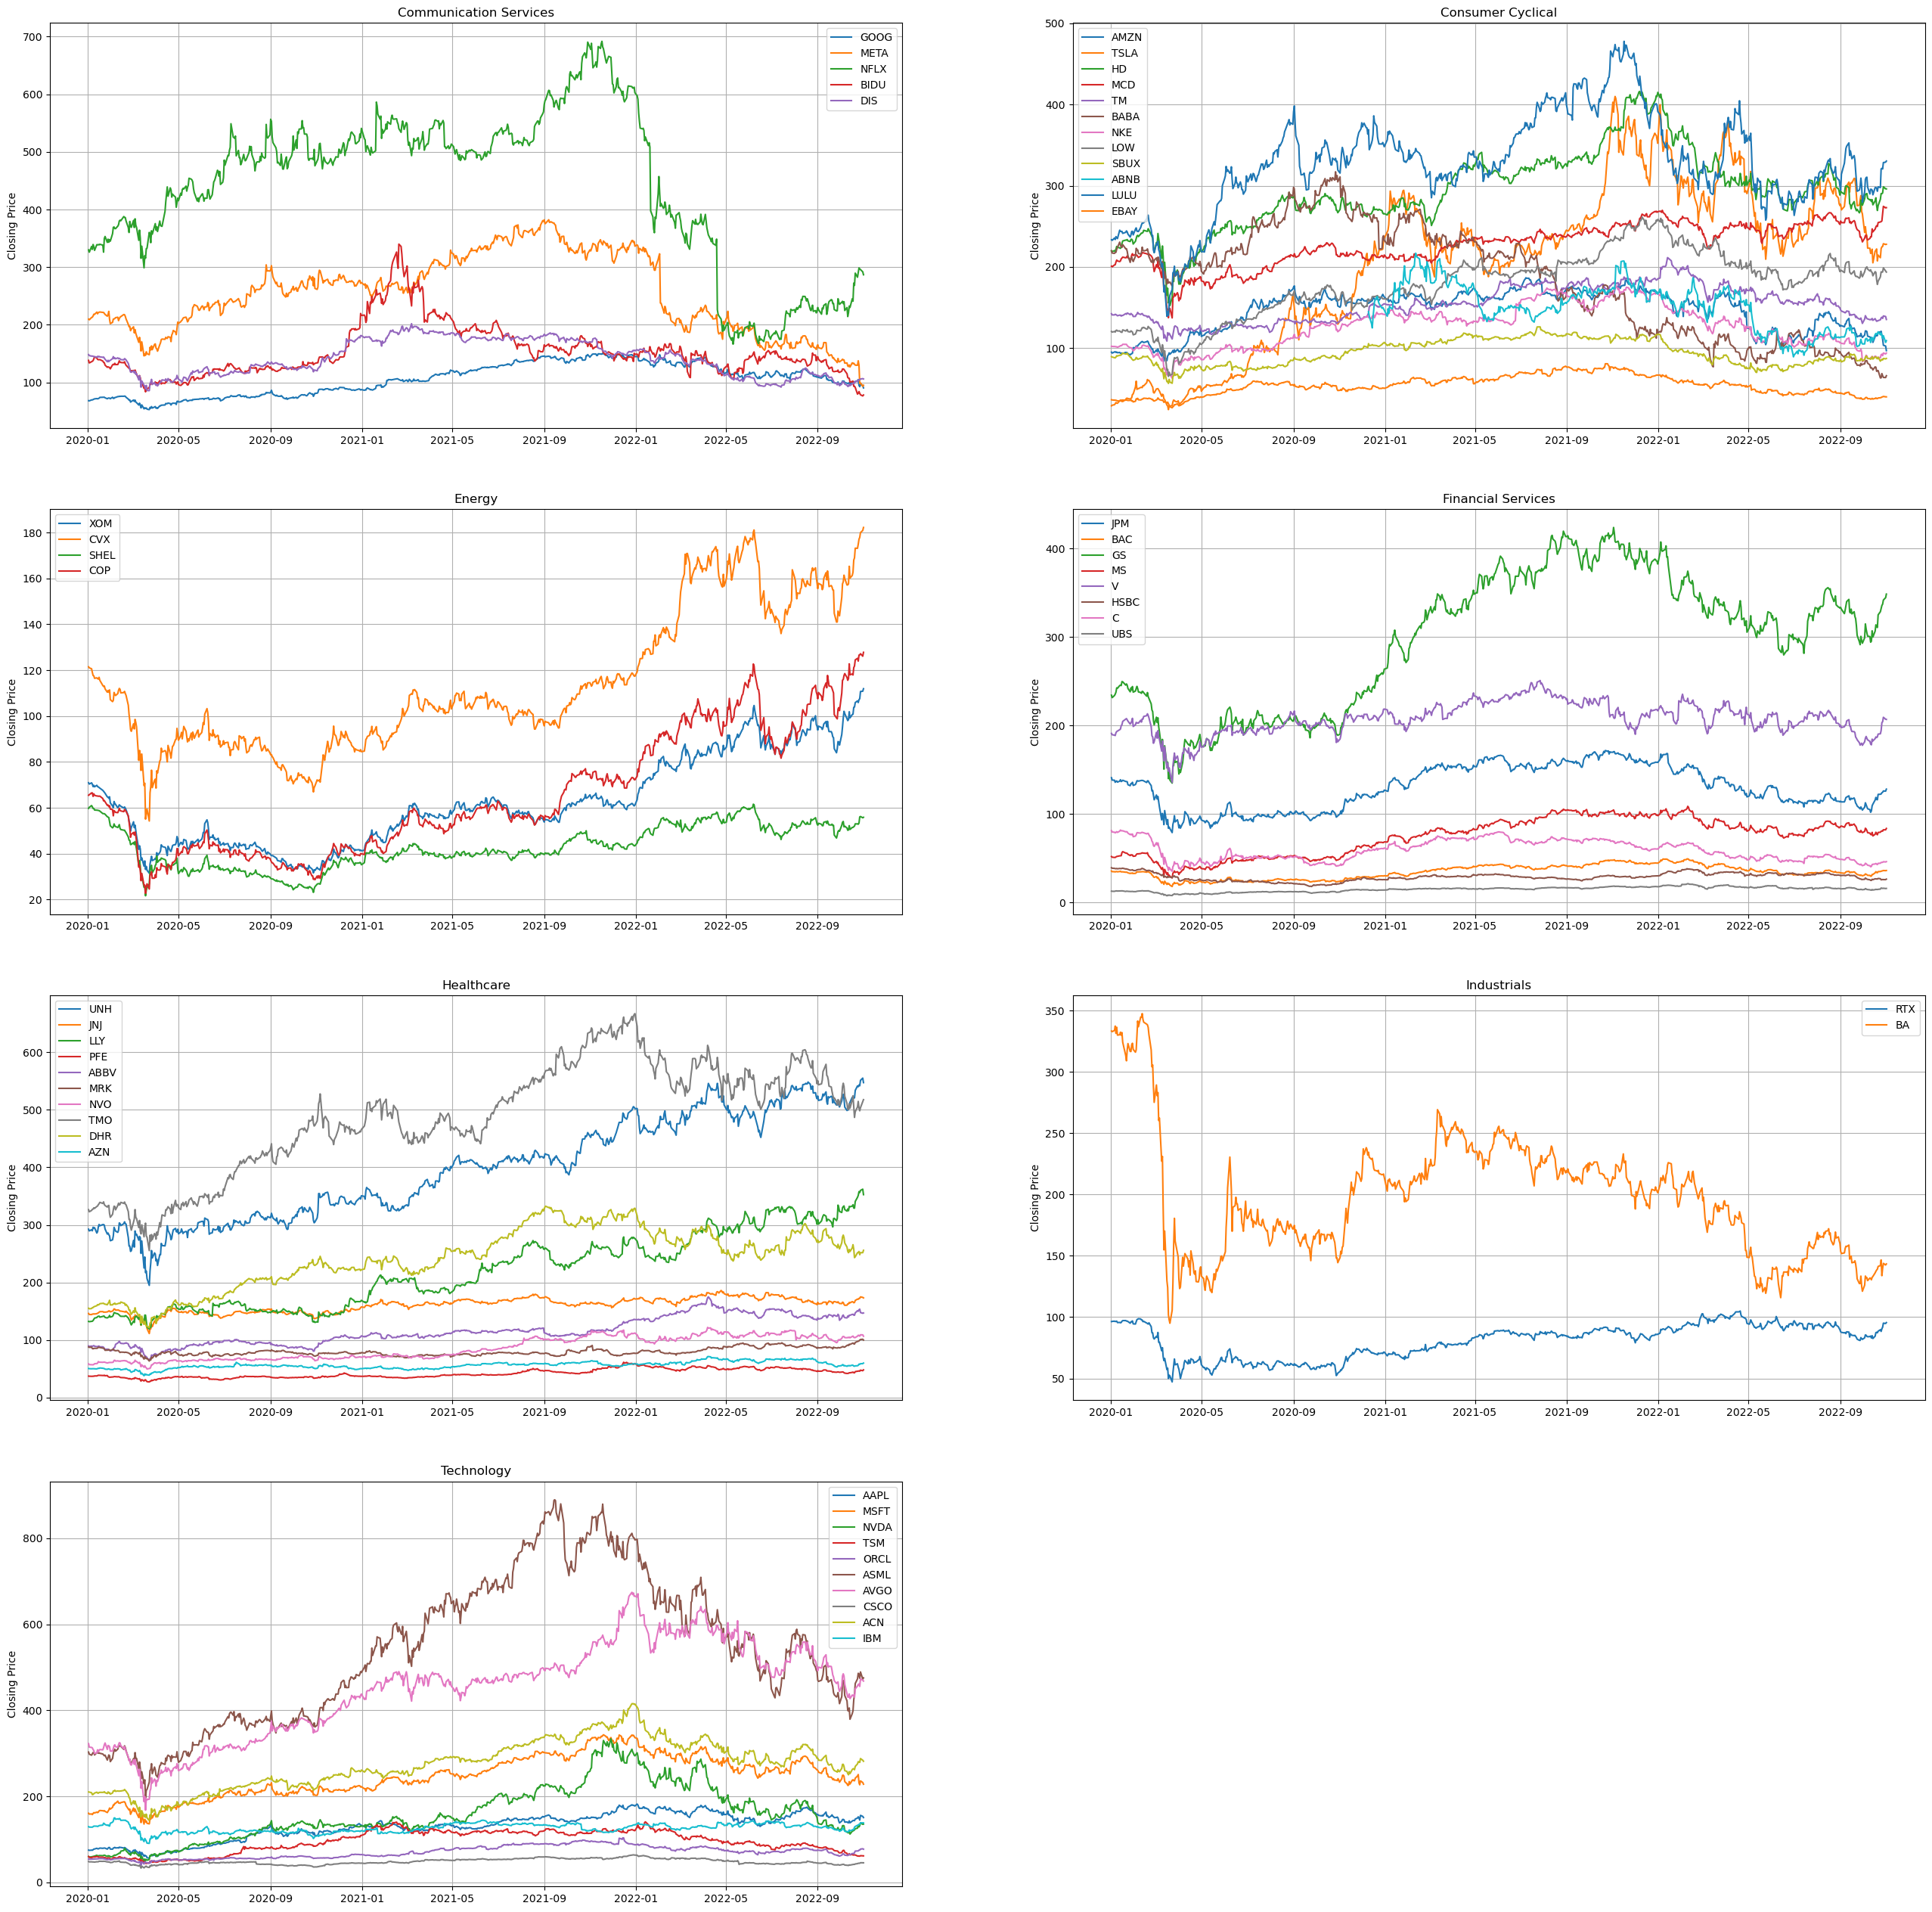
\includegraphics[scale=0.24]{figures/stocks.png}
    \caption{Stock prices in each sector.}
    \label{fig:1}
\end{figure}

We used the daily closing prices for the graph. According to IIFL Securities, “The closing price helps the investor understand the market sentiment of the stocks over time, so it is the most accurate matrix to determine the valuation of stock yearly” \cite{iifl-knowledge-center}.

The most profitable company in each sector is calculated using the average dollar volume (trading volume times closing price). We chose dollar volume as the determining factor because “money managers use dollar volume metrics to determine whether a stock has enough liquidity to support a position. It can also give us a good idea of the company's money flow when scanning for stocks” \cite{investors-underground-2019}. The company with the most dollar volume in each sector is listed below in Table~\ref{tab:1}.

\begin{table}[H]
    \centering
    \begin{tabular}{llrrr}
        \toprule
        {} & Company &       Close &        Volume &  Dollar Volume \\
        Sector                 &         &             &               &                \\
        \midrule
        Communication Services &    META &  220.07 &  2.34E+07 &   4.93E+09 \\
        Consumer Cyclical      &    TSLA &  127.00 &  1.32E+08 &   1.31E+10 \\
        Energy                 &     XOM &   68.64 &  2.04E+07 &   1.33E+09 \\
        Financial Services     &     BAC &   32.41 &  5.81E+07 &   1.83E+09 \\
        Healthcare             &     UNH &  332.38 &  3.53E+06 &   1.13E+09 \\
        Industrials            &      BA &  262.67 &  1.17E+07 &   2.54E+09 \\
        Technology             &    AAPL &   94.92 &  1.18E+08 &   1.04E+10 \\
        \bottomrule
        \end{tabular}
    \caption{Mean closing price, volume and dollar volume for each company.}
    \label{tab:1}
\end{table}

\par We chose to take a closer look at Tesla and try to make money from this stock.

%------------------------------

\subsection{Closing Price Prediction using LSTM}

Basically, in our LSTM model, we need to use $M$ days' data to predict the closing prices of the next $N$ days. Hence, we need to slide a window (with size $M+N$) across the time series data (imagine a single-variate time series for now), and then stack all the windows together into a large matrix. Figure~\ref{fig:2} illustrates this idea.

\begin{figure}[H]
    \centering
    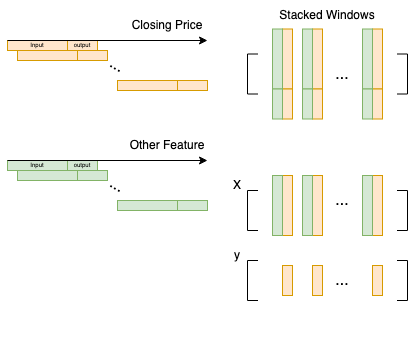
\includegraphics[scale=0.5]{figures/sliding-window.png}
    \caption{Data transformation.}
    \label{fig:2}
\end{figure}

We use the framework of PyTorch to build an LSTM model for multivariate time series, and we have also implemented a function to train the LSTM.

Note that there are a lot of hyperparameters to be determined for the LSTM. The idea is that we want to keep the inner central LSTM model as simple as possible. So, we define another class \texttt{PricePredictor} that wraps in the LSTM, and at the same time, provides all possible hyperparameters and other methods like \texttt{fit} and \texttt{predict} that will be exposed to the users.

The common methods of tuning the hyperparameters are grid search and randomized search. For grid search, we will need to fit a model for every combination of possible parameters, which is extremely time-consuming. In practice, it is preferred to use randomized search.

In our project, we intend use Scikit-lean's \texttt{RandomizedSearchCV} to do the randomized search. As described in the official documentation, our estimator / model needs to implement \texttt{fit} and \texttt{score} methods, which we have already done this in our self-defined class \texttt{PricePredictor}.

Figure~\ref{fig:3} shows predicted values v.s. observed values. It can be seen that the true closing price is very close to the predicted price, and the model fits the data quite well.

\begin{figure}[H]
    \centering
    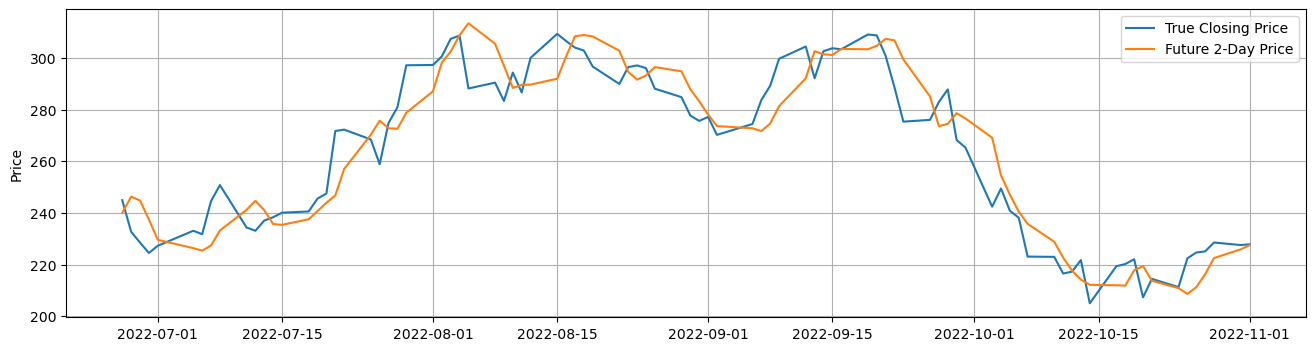
\includegraphics[scale=0.4]{figures/lstm-pred.png}
    \caption{Test result of LSTM.}
    \label{fig:3}
\end{figure}

%==============================

\section{Implementation Details and Experiment} \label{sec:3}

The mainstream trading strategies of stock trading consist of trend analysis and trading by prediction. For trend analysis, we utilized the Simple Moving Average (SMA) method and for trading by prediction, we adopted 2-days ahead prediction value by LSTM model and developed a trading strategy according to the gap between the current price and prediction price.

%------------------------------

\subsection{Simple Moving Average}

The Moving Average method is a commonly used way to smooth the price data of stocks by extracting the trending effect and excluding the fluctuation effect caused by random noise. To demonstrate this method, we need to compute the average stock price within a period of time before that day. We can slide a fixed length window (hence the name moving average) along the times series and compute the mean value of the prices falling into the window by the \textit{rolling} method from Pandas \texttt{DataFrame} (or \texttt{Series}). The trading strategy is based on the crossovers of long-term MA line and short-term MA line. The golden cross appears when the short-term MA crosses up through the long-term MA, and it indicates a signal to buy. The death cross appears when the short-term MA crosses trends down and crosses the long-term MA, and it indicates a signal to sell. We can use bitwise operations to find golden and death crosses. By definition, we note that a golden cross occurs when $\text{short-term MA} > \text{long-term MA}$ on current day, and $\text{short-term MA} < \text{long-term MA}$ on the preceding day.

The Moving Average can be constructed in different ways by selecting different parameters for Short-term and Long-term moving average lines depending on the time-horizons of traders. Commonly used lengths are 5, 10, 20, 50, 100, 200 and short length can react more sensitively to the recent changes. It can exhibit false signals and cause losing trades when the stock price is at a stable level and the MA lines are entangled with each other. Thus, to eliminate the false signals to a large extent, we chose short-term and long-term lengths to be 5 and 20 respectively. Figure~\ref{fig:4} shows the MA lines and stock price, together with the points of golden and death cross.

\begin{figure}[H]
    \centering
    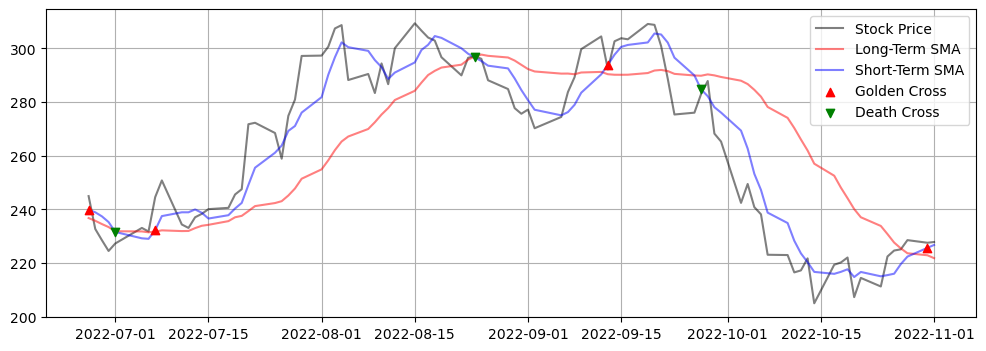
\includegraphics[scale=0.5]{figures/sma.png}
    \caption{Golden and death crosses generated by SMA.}
    \label{fig:4}
\end{figure}

To evaluate the profit by this method, we define the percentage changes by the formula
\begin{align*}
    \text{Percentage Change/ Return} = \frac{\text{Selling Price} - \text{Buying Price}}{\text{Buying Price}}
\end{align*}
And the total profit rate (out of $n$ trades) is defined as
\begin{align*}
    \text{Profit Rate} = \prod_{i=1}^n (1 +  p_i)
\end{align*}
where $p_i$ is the percentage change of the $i$-th trade.

As a result, the profit rate of investing Tesla with SMA strategy is approximately 9.19\%.

%------------------------------

\subsection{Trading by Prediction}

Another trading strategy is trading by prediction, and the prediction is made by our pre-trained LSTM model. It takes all past days before the current day into consideration and predicts the closing price $N$ days from now. This model is a method derived from Recurrent Neural Network (RNN) method, and it can solve the potential problem of RNN, thus having a better performance than RNN. Due to the unique design structure of the LSTM model, it can perform better on the process and prediction based on important events with long delay intervals. From the prediction value from previous part, we selected the 2-days ahead forecast as the prediction value and the trading strategy is that we sell the holding stock if future price is below current price while if the future price is higher than current price, we keep the holding stock and buy in more shares if having spare cash. The transaction date based on LSTM strategy is demonstrated as below in Figure~\ref{fig:5}.

\begin{figure}[H]
    \centering
    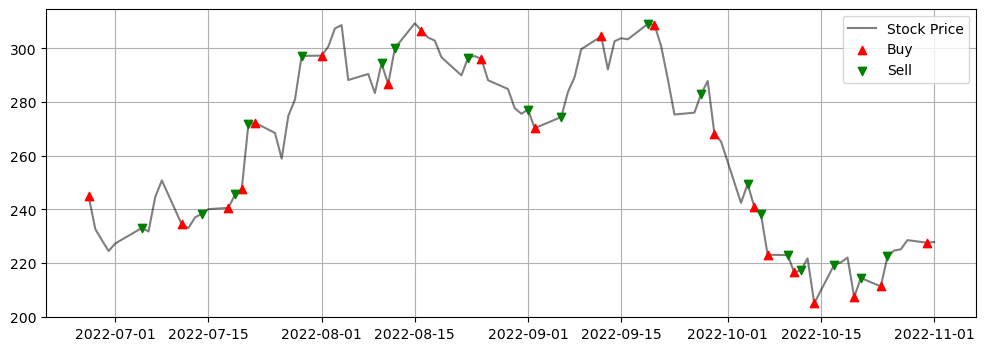
\includegraphics[scale=0.5]{figures/trade-by-pred.png}
    \caption{Dates to buy and sell.}
    \label{fig:5}
\end{figure}

The total profit rate based on LSTM prediction strategy in the last three months is 12.82\%.

Compared with the Simple Moving Average Method, the advantages of LSTM are preferable. Firstly, the trading strategy of the LSTM model is more frequent and can capture more winning opportunities than the SMA method. In addition, every transaction in the LSTM strategy is mostly profitable and can fully extract the profit space, especially when the stock price is fluctuating frequently. Finally, the SMA lines are only calculated based on historical data and have little prediction power on the future data. Sometimes the SMA signals can be random and have no instruction about the transaction.

%------------------------------

\subsection{Effective Portfolio}

In section~\ref{sec:2}, we analyzed the most profitable companies, and we can use these stocks to make the most profit out of our initial investment by creating a most effective portfolio. It is known that the weighted volatility and weighted stock returns are defined as below: 
\begin{align*}
    \text{Volatility} &= \sqrt{\mathbf{w}^\top \Sigma \mathbf{w}} \\ 
    \text{Weighted Stock Return}
    &= \mathbf{w}^\top \mathbf{r}
    = \sum_{i=1}^n w_i r_i
\end{align*}
where $\mathbf{w} = (w_1, \ldots, w_n)^\top$ is the weight assigned to each company (assuming there are $n$ companies), $r_i$ is the average stock return of the $i$-th company, and $\Sigma$ is the covariance matrix of the daily stock returns.

Now, the question is what the best weight is we invest in each profitable company. We solve this question using Monte Carlo Simulation. We generate weight for each company and select it with equal probabilities and then calculate the stock return as well as the volatility. The plot of the stock returns against the volatility for each portfolio is shown below in Figure~\ref{fig:6}.

\begin{figure}[H]
    \centering
    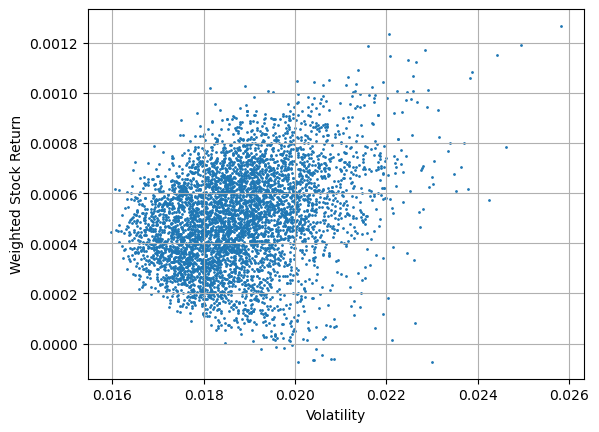
\includegraphics[scale=0.5]{figures/monte-carlo.png}
    \caption{Portfolios generated by Monte Carlo simulation.}
    \label{fig:6}
\end{figure}

We choose the most suitable portfolio referring to the Sharpe ratio, which is given by 
\begin{align*}
    \text{Shape Ratio} = \frac{\text{Stock Return}}{\text{Volatility}}
\end{align*}
We want the portfolio with the highest possible Sharpe ratio representing the return per unit of risk taken, because we want the highest return and lowest volatility. The optimal portfolio is marked as red star in Figure~\ref{fig:7}. 

\begin{figure}[H]
    \centering
    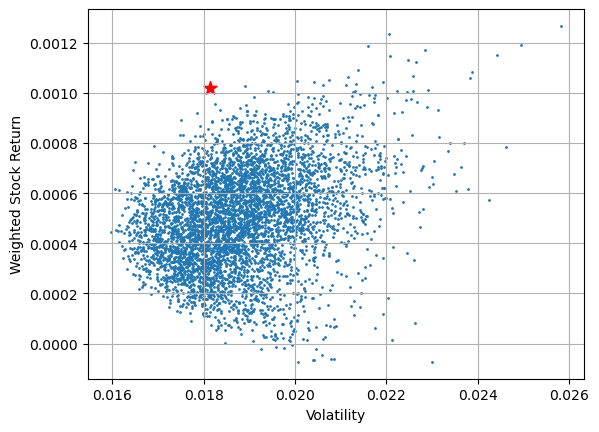
\includegraphics[scale=0.5]{figures/portfolio.png}
    \caption{Portfolio with the highest Sharpe ratio.}
    \label{fig:7}
\end{figure}

The optimal weights are listed in Table~\ref{tab:2}.

\begin{table}[H]
    \centering
    \begin{tabular}{lrrrrrrr}
        \toprule
        {} &   META &  TSLA &    XOM &   BAC &    UNH &     BA &  AAPL \\
        \midrule
        Weight & 14.70\% & 0.87\% & 25.35\% & 3.45\% & 26.79\% & 28.44\% & 0.39\% \\
        \bottomrule
        \end{tabular}
    \caption{Weight assigned to each company.}
    \label{tab:2}
\end{table}

%------------------------------

\subsection{Profits and Comparison of Trading Strategies}

To compare the two proposed strategies, we now apply the SMA strategy and prediction-based (LSTM) strategy to all seven companies. The profit rates are listed in Table~\ref{tab:3}.

\begin{table}[H]
    \centering
    \begin{tabular}{lrrrrrrr}
        \toprule
        {} &    META &   TSLA &    XOM &    BAC &   UNH &    BA &   AAPL \\
        \midrule
        SMA  & -19.97\% &  9.19\% & -2.80\% & -2.12\% & 0.77\% & 0.00\% & 17.77\% \\
        LSTM &   9.44\% & 12.82\% &  2.06\% & 11.74\% & 0.19\% & 8.91\% & 15.18\% \\
        \bottomrule
    \end{tabular}
    \caption{Profit rate of each company.}
    \label{tab:3}
\end{table}

We note that SMA performs better only for a few cases (for UNH and AAPL), while the prediction-based strategy seems to dominate SMA for most of the time. Moreover, we also observe that SMA sometimes makes us lose money. Hence, the prediction-based strategy is preferred.

Suppose we invest \$10000 to these companies with the most effective portfolio we have determined previously (Table~\ref{tab:2}), the total profits we can gain by these two strategies are shown in Table~\ref{tab:4}.

\begin{table}[H]
    \centering
    \begin{tabular}{lrrrrrrr rr}
        \toprule
        {} &   META &  TSLA &    XOM &    BAC &    UNH &     BA &  AAPL & Total Rate & Total Profit\\
        \midrule
        Weight        & 14.70\% & 0.87\% & 25.35\% &  3.45\% & 26.79\% & 28.44\% & 0.39\% \\
        SMA  & -2.94\% & 0.08\% & -0.71\% & -0.07\% &  0.21\% &  0.00\% & 0.07\% & -3.36\% & -336.22 \\
        LSTM &  1.39\% & 0.11\% &  0.52\% &  0.41\% &  0.05\% &  2.54\% & 0.06\% &  5.07\% & 507.27\\
        \bottomrule
    \end{tabular}
    \caption{Weighted profit rate of each company and the total profit.}
    \label{tab:4}
\end{table}

As we can see, if we apply SMA strategy, we will end up losing \$336.62. However, if we use prediction-based strategy, we will earn \$507.27.

%==============================

\section{News Investigation} \label{sec:4}

%------------------------------

\subsection{Searching Google by URL}

When typing something into Google's search bar, essentially, we are creating a URL which leads to a website. For example, the following URL will lead to the webpage that we can reach by typing the word apple into the search bar. Note that we can do so much more than just search based on a string (search bar input), which is basically what we usually do. In addition, we can add parameters to the URL so that more constraints on our search are specified. For example, we can search news within a particular date range.
We refer to this link\cite{stenevang-2016} for some detailed information about Google's search URL request parameters.
Some parameters of interest:

\begin{enumerate}
    \item \texttt{tbm}, TBM (Term By Method), e.g., \texttt{tbm=nws} will search for news
    \item \texttt{tbs}, TBS (Term By Search), e.g.,
    \begin{enumerate}
        \item \verb|tbs=cdr:1,cd_min:3/2/1984,cd_max:6/5/1987| specifies a range from March 2, 1984, to June 5, 1987
        \item \texttt{tbs=sbd:0} sorts the results by relevance
    \end{enumerate}
    \item \texttt{lr}, language, e.g.
    \begin{enumerate}
        \item \verb|lr=lang_en| for English
        \item \verb|lr=lang_zh-CN| for Chinese
    \end{enumerate}
\end{enumerate}

If we want to search news about Tesla on October 1, 2022, then the URL is: 

\begin{lstlisting}
https://www.google.com/search?q=Tesla&tbm=nws&tbs=cdr:1,cd_min:10/01/2022,cd_max:10/01/2022,sbd:0&lr=lang_en
\end{lstlisting}

\subsection{Find Links to Webpages and Scraping Headlines}

Next, we can use the function \texttt{requests.get} to request the content of a website to transform the link to a webpage. One thing to notice is that we must always remember to add a header to pretend to be a browser, otherwise our request may be denied.

\begin{lstlisting}[language=python]
headers = { 
    "User-Agent": "Mozilla/5.0 (Macintosh; Intel Mac OS X 10.15; rv:106.0) Gecko/20100101 Firefox/106.0"
}
res = requests.get(url, headers=headers)
# res should be <Response [200]>
\end{lstlisting}

The return code 200 means that the request is successful. We parse the raw HTML content using \texttt{bs4.BeautifulSoup}. By observing the HTML structure of the Google search page, we find that all links are contained inside tags with \texttt{class=SoaBEf} (see the screenshot in Figure~\ref{fig:8}). And these tags are descendants of a tag with \texttt{id=search}.

\begin{figure}[H]
    \centering
    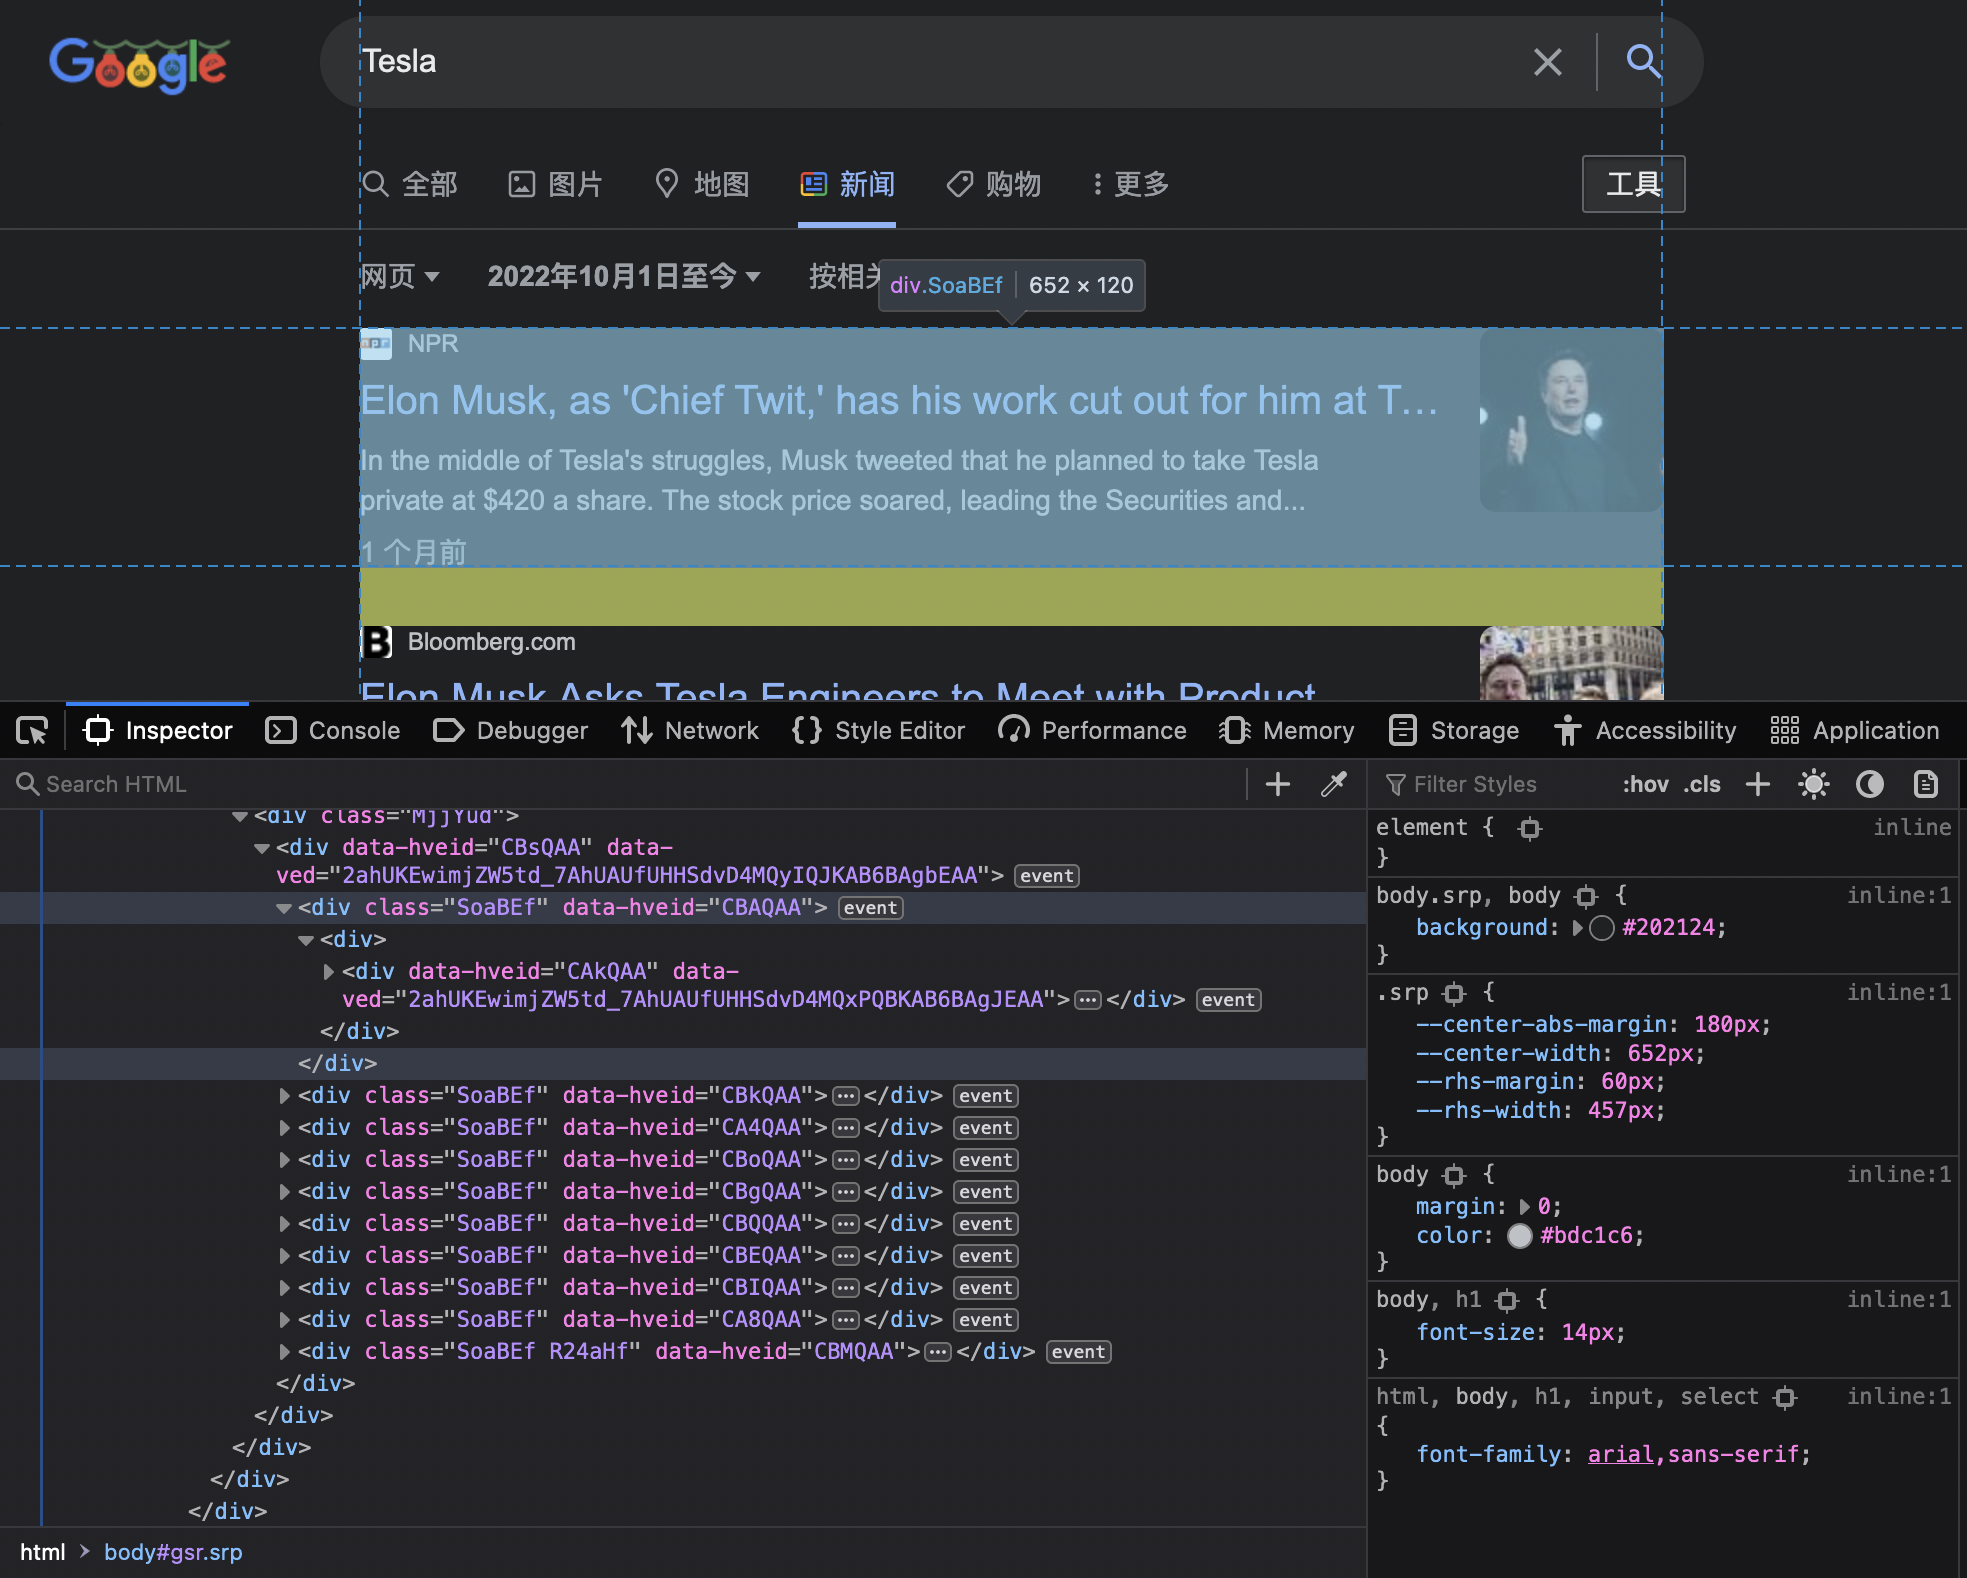
\includegraphics[scale=0.4]{figures/weblink.png}
    \caption{Screenshot of browser console.}
    \label{fig:8}
\end{figure}

The news headline is often the first heading of a news webpage, which is contained in a \texttt{<h1>} HTML tag. For example, we found a headline from a webpage about Tesla, \texttt{'Tesla boss Elon Musk presents humanoid robot Optimus'}.

In our command line app \texttt{main.py}, we have implemented a command \texttt{find-company-new} that can automatically search for news headlines and then store them in a SQLite database. For example, we can find the news for Tesla from October 1, 2022, to October 5, 2022, in a terminal via:
\begin{lstlisting}[language=sh]
> python main.py find-company-news --company TSLA --query "Tesla" --from-date "2022-10-1" --to-date "2022-10-5" --force
Start searching for news headlines...
News on 2022-10-01: Tesla boss Elon Musk presents humanoid robot Optimus
News on 2022-10-02: Tesla blames logistics problems after delivering fewer cars than forecast
News on 2022-10-03: Tesla slides on widening delivery and production gap, demand worries
News on 2022-10-04: A Musk Retweet: Tesla CEO Says He'll Pay $44 Billion to Buy Twitter
News on 2022-10-05: Musk's move to close Twitter deal leaves Tesla investors worried
Successfully found all the news for TSLA.
\end{lstlisting}

\subsection{Quantification of New Scrapping}

The quantification of the news scrapping is to use the mechanism of word embedding. The word embedding used the pre-trained model provided by module \verb|sentence_transformers|. The detailed discussion can be found in our webpage\footnote{\url{https://isaac-fate.github.io/stox/news-investigation/quantification.html}}.

%==============================

\section{Conclusion}

To apply the trading strategy, we have to develop an LSTM prediction model for the stock price.

In our trading strategy, we used two methods. They are simple moving averages and trading by prediction trading method. A simple moving average with short length 5 and long length 20 is adopted. When the short SMA is bigger than the long SMA, we buy the stock, vice versa. Next, a 2-day ahead forecast as the predicted value LSTM model is adopted, and we buy the stock if the future price is above current price, vice versa. Using Tesla stock price as training data, the profit rate from the earlier model is 9\%, and the profit rate using the later model is 12\%. Therefore, for TESLA stock, LSTM trading strategy is better. Our team also developed an optimal portfolio using the most profitable stocks in each sector. The idea is to find the portfolio with the lowest volatility and highest return in Monte Carlo simulation.

The news scraping method is developed to draw the content from internet that explains the stock change. The mechanism is start from search Google by URL, and from URL to webpages, and finally from webpage to Scrape Headline. 

However, there is limitation in our trading strategy. The parameter in SMA method is manually selected by observing. One improvement is that we can use machine learning method to select the parameter for short SMA and long SMA automatically based on the historical data.

Another limitation is that the LSTM model is based on the training data that can minimize the model standard error, but an improvement could be using the training data that can generate most profit to predict future stock prices. That is to combine the LSTM model for prediction and the objective, which is to optimize the profit, together. 

The prediction using news scrapping has limitation because use SVM to predict the rise or fall of tomorrow's stock price gives us an AUC index of 0.51, which is low.

%==============================

\printbibliography

%==============================

\appendix
\appendixpage
\addappheadtotoc

\section{Contribution}

\begin{table}[H]
    \centering
    \begin{tabular}{l l p{10cm}}
        \toprule
        Name & ID & \multicolumn{1}{c}{Contribution}\\
        \midrule
        FEI Yiheng
        & 3036044533
        & \begin{itemize}
            \item Set up the project and organized the documentation on the website
            \item Implemented and trained LSTM model by randomized search
            \item Composed a script to scrape news headlines and did rough analysis with word embedding and SVM
        \end{itemize}\\
        HE Zeyu 
        & 3036043620
        & \begin{itemize}
            \item Made PowerPoint and presentation
            \item Composed 3.1 and 3.2 of the report
        \end{itemize} \\ 
        LI Ziwan
        & 3036043852
        & \begin{itemize}
            \item Composed the report
            \item Discussed the trading strategy with team members 
            \item Shared financial knowledge with teammates without finance backgrounds
        \end{itemize}\\
        LI Yuhan
        & 3035914729
        & \begin{itemize}
            \item Collected and preprocessed data 
            \item Plotted stock price trend sector by sector and conducted visualization
        \end{itemize} \\ 
        SHI Keyan
        & 3036044002
        & \begin{itemize}
            \item Implemented strategy of assigning weights for stocks (Optimal Stock Portfolio)
            \item Participated in designing and implementing the trading strategies
        \end{itemize} \\
        YI Xunming
        & 3036044430
        & \begin{itemize}
            \item Built several models to predict the future stock prices
            \item Created a reasonable strategy model
        \end{itemize} \\ 
        \bottomrule
    \end{tabular}
\end{table}

%------------------------------

\section{GitHub Repository and Webpage}

\url{https://github.com/Isaac-Fate/stox}

\url{https://isaac-fate.github.io/stox}

%------------------------------

\section{Presentation URL}

\url{https://www.youtube.com/watch?v=N-pbX9vEjZ8}

%==============================

\end{document}